

\tikzset{every picture/.style={line width=0.3pt}} %set default line width to 0.75pt        

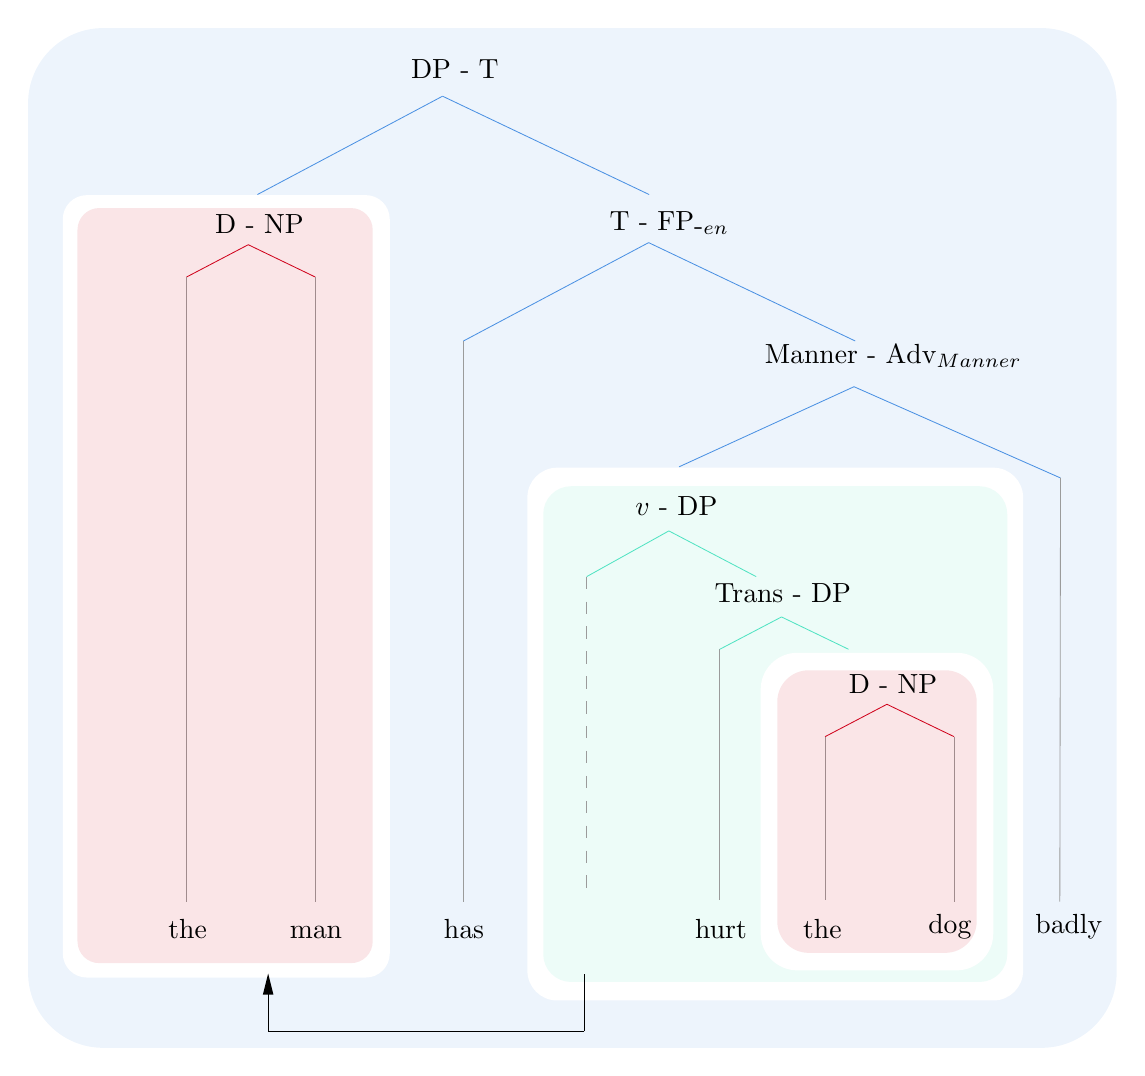
\begin{tikzpicture}[x=0.75pt,y=0.75pt,yscale=-0.85,xscale=0.85]
%uncomment if require: \path (0,709); %set diagram left start at 0, and has height of 709

%Rounded Rect [id:dp034885216520763374] 
\draw  [draw opacity=0][fill={rgb, 255:red, 74; green, 144; blue, 226 }  ,fill opacity=0.1 ] (88,80.93) .. controls (88,57.41) and (107.07,38.33) .. (130.6,38.33) -- (662.4,38.33) .. controls (685.93,38.33) and (705,57.41) .. (705,80.93) -- (705,573.73) .. controls (705,597.26) and (685.93,616.33) .. (662.4,616.33) -- (130.6,616.33) .. controls (107.07,616.33) and (88,597.26) .. (88,573.73) -- cycle ;
%Rounded Rect [id:dp864413197045051] 
\draw  [draw opacity=0][fill={rgb, 255:red, 255; green, 255; blue, 255 }  ,fill opacity=1 ] (371,304.4) .. controls (371,295.07) and (378.57,287.5) .. (387.9,287.5) -- (635.1,287.5) .. controls (644.43,287.5) and (652,295.07) .. (652,304.4) -- (652,572.6) .. controls (652,581.93) and (644.43,589.5) .. (635.1,589.5) -- (387.9,589.5) .. controls (378.57,589.5) and (371,581.93) .. (371,572.6) -- cycle ;
%Rounded Rect [id:dp31861860103211814] 
\draw  [draw opacity=0][fill={rgb, 255:red, 80; green, 227; blue, 194 }  ,fill opacity=0.1 ] (380,313.82) .. controls (380,305.08) and (387.08,298) .. (395.82,298) -- (627.18,298) .. controls (635.92,298) and (643,305.08) .. (643,313.82) -- (643,563.18) .. controls (643,571.92) and (635.92,579) .. (627.18,579) -- (395.82,579) .. controls (387.08,579) and (380,571.92) .. (380,563.18) -- cycle ;
%Rounded Rect [id:dp23576358575832845] 
\draw  [draw opacity=0][fill={rgb, 255:red, 255; green, 255; blue, 255 }  ,fill opacity=1 ] (503.24,413.2) .. controls (503.24,401.72) and (512.55,392.42) .. (524.03,392.42) -- (614.3,392.42) .. controls (625.78,392.42) and (635.08,401.72) .. (635.08,413.2) -- (635.08,551.63) .. controls (635.08,563.11) and (625.78,572.42) .. (614.3,572.42) -- (524.03,572.42) .. controls (512.55,572.42) and (503.24,563.11) .. (503.24,551.63) -- cycle ;
%Rounded Rect [id:dp7324546519566175] 
\draw  [draw opacity=0][fill={rgb, 255:red, 255; green, 255; blue, 255 }  ,fill opacity=1 ] (107.67,146.66) .. controls (107.67,139.12) and (113.78,133) .. (121.33,133) -- (279.34,133) .. controls (286.88,133) and (293,139.12) .. (293,146.66) -- (293,562.84) .. controls (293,570.38) and (286.88,576.5) .. (279.34,576.5) -- (121.33,576.5) .. controls (113.78,576.5) and (107.67,570.38) .. (107.67,562.84) -- cycle ;
%Straight Lines [id:da3972557940014332] 
\draw [color={rgb, 255:red, 208; green, 2; blue, 27 }  ,draw opacity=1 ]   (250.8,179.44) -- (212.8,161.11) ;
%Straight Lines [id:da3734280152933176] 
\draw [color={rgb, 255:red, 208; green, 2; blue, 27 }  ,draw opacity=1 ]   (212.8,161.11) -- (177.8,179.44) ;
%Straight Lines [id:da8957091119411691] 
\draw [color={rgb, 255:red, 208; green, 2; blue, 27 }  ,draw opacity=1 ]   (612.8,439.93) -- (574.8,421.6) ;
%Straight Lines [id:da8730392291245619] 
\draw [color={rgb, 255:red, 208; green, 2; blue, 27 }  ,draw opacity=1 ]   (574.8,421.6) -- (539.8,439.93) ;
%Straight Lines [id:da36657403374376774] 
\draw [color={rgb, 255:red, 155; green, 155; blue, 155 }  ,draw opacity=1 ]   (539.8,439.93) -- (539.8,532.6) ;
%Straight Lines [id:da11962397518947854] 
\draw [color={rgb, 255:red, 155; green, 155; blue, 155 }  ,draw opacity=1 ]   (612.8,439.93) -- (612.8,533.4) ;
%Straight Lines [id:da4999235058666789] 
\draw [color={rgb, 255:red, 155; green, 155; blue, 155 }  ,draw opacity=1 ]   (480.05,390.43) -- (480.05,532.6) ;
%Straight Lines [id:da6548410354329881] 
\draw [color={rgb, 255:red, 80; green, 227; blue, 194 }  ,draw opacity=1 ]   (553.05,390.43) -- (515.05,372.1) ;
%Straight Lines [id:da2235852996451071] 
\draw [color={rgb, 255:red, 80; green, 227; blue, 194 }  ,draw opacity=1 ]   (515.05,372.1) -- (480.05,390.43) ;
%Straight Lines [id:da0769185876775682] 
\draw [color={rgb, 255:red, 80; green, 227; blue, 194 }  ,draw opacity=1 ]   (500.65,349.23) -- (451.2,323.33) ;
%Straight Lines [id:da7127264168717515] 
\draw [color={rgb, 255:red, 80; green, 227; blue, 194 }  ,draw opacity=1 ]   (451.2,323.33) -- (404.65,349.23) ;
%Straight Lines [id:da1867123098813408] 
\draw [color={rgb, 255:red, 155; green, 155; blue, 155 }  ,draw opacity=1 ] [dash pattern={on 4.5pt off 4.5pt}]  (404.65,349.23) -- (404.65,532.5) ;
%Straight Lines [id:da4924213637331023] 
\draw [color={rgb, 255:red, 74; green, 144; blue, 226 }  ,draw opacity=1 ]   (673.2,293.33) -- (556.13,241.6) ;
%Straight Lines [id:da3715548654487917] 
\draw [color={rgb, 255:red, 74; green, 144; blue, 226 }  ,draw opacity=1 ]   (556.13,241.6) -- (457,287) ;
%Straight Lines [id:da022458887362470925] 
\draw [color={rgb, 255:red, 155; green, 155; blue, 155 }  ,draw opacity=1 ]   (673.2,293.33) -- (672.8,533.4) ;
%Straight Lines [id:da084129560695545] 
\draw [color={rgb, 255:red, 155; green, 155; blue, 155 }  ,draw opacity=1 ]   (334.8,215.67) -- (334.8,533.4) ;
%Straight Lines [id:da11283861445316812] 
\draw [color={rgb, 255:red, 74; green, 144; blue, 226 }  ,draw opacity=1 ]   (556.8,215.67) -- (439.73,159.93) ;
%Straight Lines [id:da18405698017218852] 
\draw [color={rgb, 255:red, 74; green, 144; blue, 226 }  ,draw opacity=1 ]   (439.73,159.93) -- (334.8,215.67) ;
%Straight Lines [id:da4142916860805901] 
\draw [color={rgb, 255:red, 155; green, 155; blue, 155 }  ,draw opacity=1 ]   (250.8,179.44) -- (250.8,533.4) ;
%Straight Lines [id:da9820239195731701] 
\draw [color={rgb, 255:red, 155; green, 155; blue, 155 }  ,draw opacity=1 ]   (177.8,179.44) -- (177.8,533.4) ;
%Straight Lines [id:da8912900354325306] 
\draw [color={rgb, 255:red, 74; green, 144; blue, 226 }  ,draw opacity=1 ]   (440,132.67) -- (322.93,76.93) ;
%Straight Lines [id:da46428872338489646] 
\draw [color={rgb, 255:red, 74; green, 144; blue, 226 }  ,draw opacity=1 ]   (322.93,76.93) -- (218,132.67) ;
%Straight Lines [id:da27398889935539716] 
\draw    (403.27,606.8) -- (224.07,606.8) ;
%Straight Lines [id:da6293499120506956] 
\draw    (403.27,606.8) -- (403.27,574.2) ;
%Straight Lines [id:da1448979089622664] 
\draw    (224.07,606.8) -- (224.07,576.2) ;
\draw [shift={(224.07,574.2)}, rotate = 90] [fill={rgb, 255:red, 0; green, 0; blue, 0 }  ][line width=0.08]  [draw opacity=0] (12,-3) -- (0,0) -- (12,3) -- cycle    ;
%Rounded Rect [id:dp49028218668622503] 
\draw  [draw opacity=0][fill={rgb, 255:red, 208; green, 2; blue, 27 }  ,fill opacity=0.1 ] (116,152.67) .. controls (116,145.86) and (121.52,140.33) .. (128.33,140.33) -- (271,140.33) .. controls (277.81,140.33) and (283.33,145.86) .. (283.33,152.67) -- (283.33,556) .. controls (283.33,562.81) and (277.81,568.33) .. (271,568.33) -- (128.33,568.33) .. controls (121.52,568.33) and (116,562.81) .. (116,556) -- cycle ;
%Rounded Rect [id:dp8649953827045236] 
\draw  [draw opacity=0][fill={rgb, 255:red, 208; green, 2; blue, 27 }  ,fill opacity=0.1 ] (512.66,420.15) .. controls (512.66,410.31) and (520.64,402.33) .. (530.47,402.33) -- (607.85,402.33) .. controls (617.69,402.33) and (625.67,410.31) .. (625.67,420.15) -- (625.67,544.69) .. controls (625.67,554.52) and (617.69,562.5) .. (607.85,562.5) -- (530.47,562.5) .. controls (520.64,562.5) and (512.66,554.52) .. (512.66,544.69) -- cycle ;

% Text Node
\draw (178.41,556) node [anchor=south] [inner sep=0.75pt]   [align=left] {the};
% Text Node
\draw (251.16,556) node [anchor=south] [inner sep=0.75pt]   [align=left] {man};
% Text Node
\draw (335.07,556) node [anchor=south] [inner sep=0.75pt]   [align=left] {has};
% Text Node
\draw (480.76,556) node [anchor=south] [inner sep=0.75pt]   [align=left] {hurt};
% Text Node
\draw (538.21,556) node [anchor=south] [inner sep=0.75pt]   [align=left] {the};
% Text Node
\draw (610.47,556) node [anchor=south] [inner sep=0.75pt]   [align=left] {dog};
% Text Node
\draw (677.91,556) node [anchor=south] [inner sep=0.75pt]   [align=left] {badly};
% Text Node
\draw (551.8,403.27) node [anchor=north west][inner sep=0.75pt]   [align=left] {D - NP};
% Text Node
\draw (475.8,351.52) node [anchor=north west][inner sep=0.75pt]   [align=left] {Trans - DP};
% Text Node
\draw (430.8,302.32) node [anchor=north west][inner sep=0.75pt]   [align=left] {$\displaystyle v$ - DP};
% Text Node
\draw (504.2,216) node [anchor=north west][inner sep=0.75pt]   [align=left] {Manner - Adv$\displaystyle _{\text{Manner}}$};
% Text Node
\draw (416.2,140.8) node [anchor=north west][inner sep=0.75pt]   [align=left] {T - FP$\displaystyle _{\text{\mbox{-}en}}$};
% Text Node
\draw (192.67,142.44) node [anchor=north west][inner sep=0.75pt]   [align=left] {D - NP};
% Text Node
\draw (303.67,54.6) node [anchor=north west][inner sep=0.75pt]   [align=left] {DP - T};


\end{tikzpicture}
